% ==============================================================================
% РАЗДЕЛ 2.2: Оценка переходного процесса и влияния различных факторов
% Партия B03-019 (DISS-005-B0813 .. DISS-005-B0861, 49 блоков)
% ==============================================================================


(Примечание автора: Закрываем примечание 3 "Взято из статей про КР", не надо ответа на это сообщение)

% DISS-005-B0813
\subsection{Оценка переходного процесса и влияния различных факторов}
\label{sec:ch02_transient_and_harmonics}


(Примечание автора: А чего не поправила (Рисунок 2.5)? Пройдис по всем похожим паттернам и поправь их, где это нужно, может где-то будет "рис.", а где-то "РИС." и т.д.(Рисунок 2.6))
% DISS-005-B0814
Мы можем видеть (Рисунок 2.5), что для классических ТТ, при наличии апериодической составляющей в первичном токе, довольно длительное время сохраняются колебания (127~мс). Для катушек Роговского, данный недостаток практически отсутствует, что особенно ярко видно при построении годографа векторов тока (рисунок~\ref{fig:ch02_hodograph}). Годограф отображает траекторию движения вектора, который используется для работы различных направленных защит, например, РНМ в устройствах БАВР.

% DISS-005-B0815
В случае применения КР, вектор из точки с нулевым током (точка 1, Рисунок 2.6) достигает установившегося значения (точка 2, Рисунок 2.6) за время, равное периоду промышленной частоты (20~мс). При этом траектория движения вектора, рассчитанного на основе этого сигнала, не зависит от угла КЗ.

% DISS-005-B0816
Хотя классические ТТ могут достигать близкого значения быстрее ($\varphi_{\text{КЗ}} = 0$)~-- за 15~мс (около точки 2, Рисунок 2.6)\commentnote{DISS-005-C0077}{Андрей Яблоков}{Вот это не сходится с рисунком вроде, все годографы кроме темно синего достигает точки 3 быстрее. Надо как то пояснить мысль, читатель не поймет}\commentnote{DISS-005-C0078}{Алексей Евдаков}{Переписал. Ибо суть в том, что у\textbackslash\textbackslash КР -- траектория стабильна и одинакова\textbackslash\textbackslash ТТ -- траектория изменяется от момента начала аварии}, но в этом случае вектор колеблется вокруг точки установившегося значения ещё длительное время, и входит в допустимый диапазон только через 127~мс от начала процесса (точка 2, Рисунок 2.5). При других углах КЗ время переходного процесса изменяется, и в случае отсутствия апериодической составляющей ($\varphi_{\text{КЗ}} = 90$) может быть аналогично с КР, то есть достигать установившегося значения (точка 2 на рисунке~\ref{fig:ch02_hodograph}) за период промышленной частоты (20~мс).

(Примечание автора: Закрываем примечание 4 ("Вот это не сходится с...") и 5 ("Переписал. Ибо суть в том..."), не надо ответа на это сообщение)

% DISS-005-B0817
Таким образом, у классических ТТ, в зависимости от момента начала аварии ($\varphi_{\text{КЗ}}$), наблюдается непостоянство траектории движения вектора тока и времени переходного процесса. В отличие от них, применение КР позволяет избежать этой неоднозначности, обеспечивая более стабильное и предсказуемое поведение защит.

% DISS-005-B0818
% DISS-005-B0819
\begin{figure}[htbp]
  \centering
  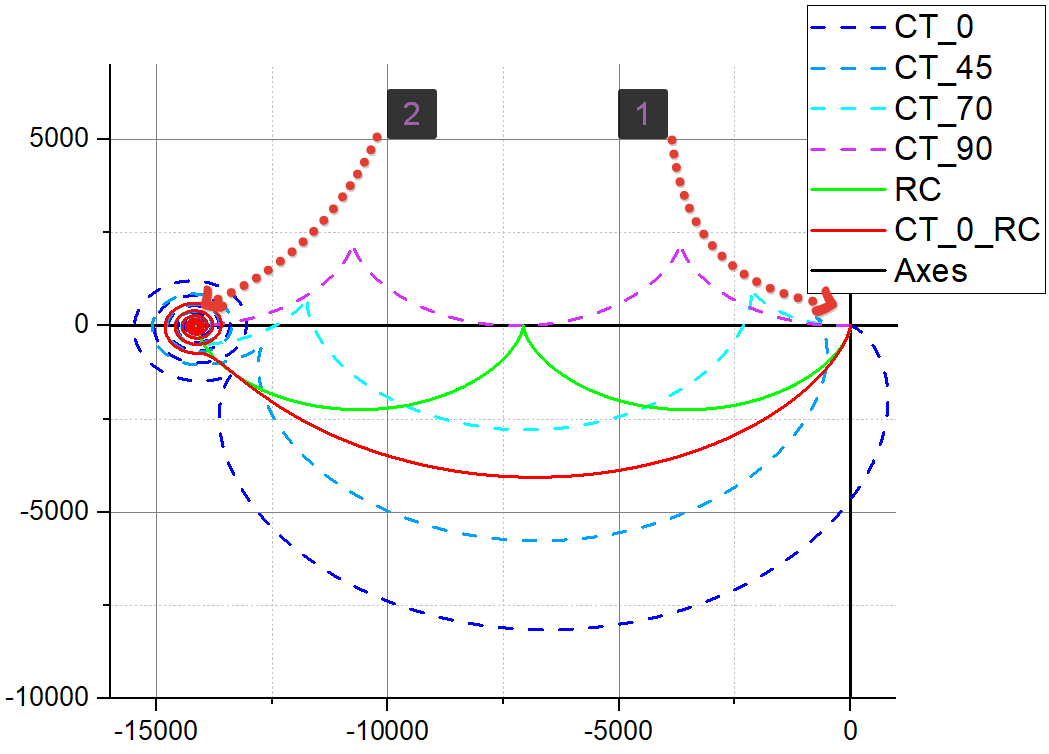
\includegraphics[width=0.85\textwidth]{image60.png}
  \caption{Годограф вектора тока получаемого с классических ТТ при различных углах КЗ (CT\_0 -- CT\_90) с учётом корректировки по углу, с КР, а также усреднённого сигнала при максимальной доли апериодики. Точка 1~-- начало процесса, точка 2~-- окончание процесса.}
  \label{fig:ch02_hodograph}
\end{figure}

% DISS-005-B0820
\paragraph{Влияние постоянной времени затухания ($\tau_0$).}

% DISS-005-B0821
Доля апериодической составляющей была задана максимальной ($\varphi_{\text{КЗ}} = 0$), а все иные параметры, участвующие в формуле~\eqref{eq:kz_current}\commentnote{DISS-005-C0079}{Андрей Яблоков}{Надо описать где то, что это за иные параметры исходной модели}\commentnote{DISS-005-C0080}{Алексей Евдаков}{Пока не придумал, как лучше. Да и\dots\ других параметров особо нет. Это скорее совсем базовые, например частота сети, длина процесса и т.д.}\commentnote{DISS-005-C0081}{Андрей Яблоков}{Может сослаться на формулу: все иные параметры тока, участвующие в формуле 1, \dots.}\commentnote{DISS-005-C0082}{Алексей Евдаков}{Да, спасибо за идею.}, оставлены исходными для данной модели. Как можем видеть, на всём промежутке значений $\tau_0$: от 1~мс до 700~мс, что охватывает все встречаемые на практике значения параметра (от 1~мс до 540~мс согласно [24]), использование КР даёт либо лучшее время переходного процесса, либо соизмеримое (Рисунок 2.7~а,~б). Причём, при постоянных времени более 40~мс, время переходного процесса определяется исключительно математическими факторами и особенностями БПФ и равно 20~мс. Классические же ТТ могут достигать времени переходного процесса равного порядка 240~мс. При этом, стоит не забывать, что трансформаторы тока с ферромагнитными сердечниками часто успевают насытиться за это время, и их показания окажутся ещё хуже, чем представленные здесь для идеального сигнала.

(Примечание автора: Закрываем примечание 6, 7, 8, 9 и не надо ответа на это сообщение)

% DISS-005-B0822
\paragraph{Влияние начального угла КЗ.}

% DISS-005-B0823
Переменная $\tau_0$ была задана равной 50~мс, все остальные параметры оставлены стандартными. Можем видеть (Рисунок 2.7~в,г), что чем больше доля апериодической составляющей (чем ближе угол КЗ к 0), тем это искажение сильнее у классических ТТ. Для КР же, при данной $\tau_0$, время переходного процесса определяется исключительно математическими факторами, как и было показано ранее.

% DISS-005-B0824
\paragraph{Влияние частоты дискретизации.}

% DISS-005-B0825
По результатам моделирования получено, что количество выборок на период не оказывает существенного влияния на точность измерения при стандартных значениях (20, 24, 32, 48, 96 и более).

% DISS-005-B0826
% DISS-005-B0827
% DISS-005-B0828
% DISS-005-B0829
% DISS-005-B0830
% DISS-005-B0831
% DISS-005-B0832
% DISS-005-B0833
% DISS-005-B0834
% DISS-005-B0835
% DISS-005-B0836
\begin{figure}[htbp]
  \centering
  \begin{tabular}{cc}
    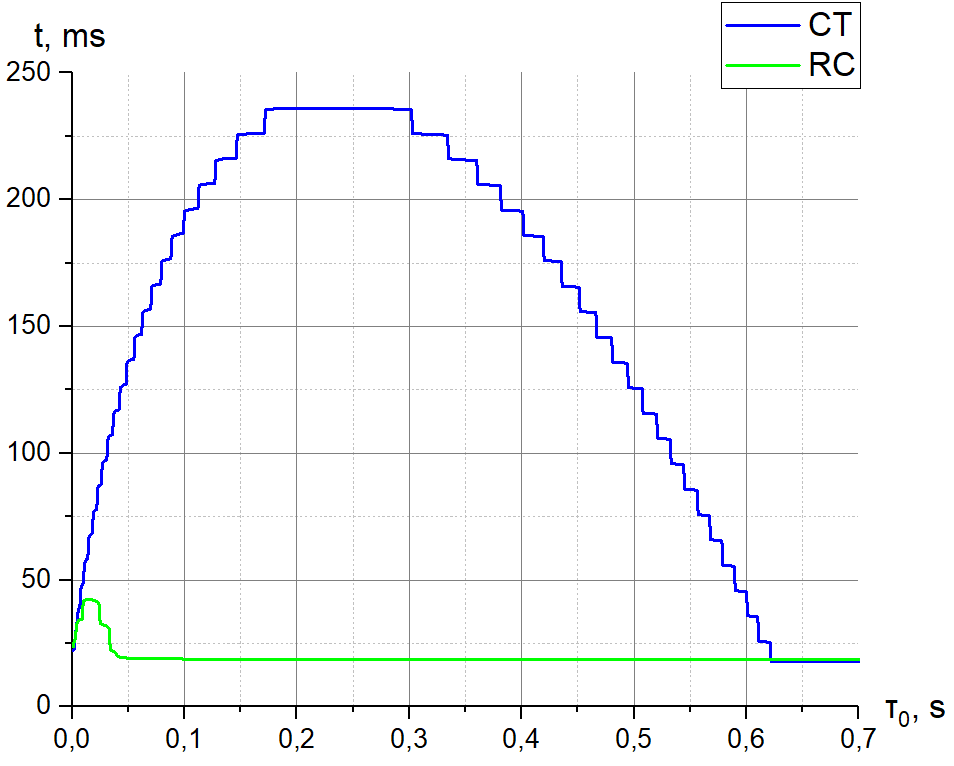
\includegraphics[width=0.46\textwidth]{image61.png} & 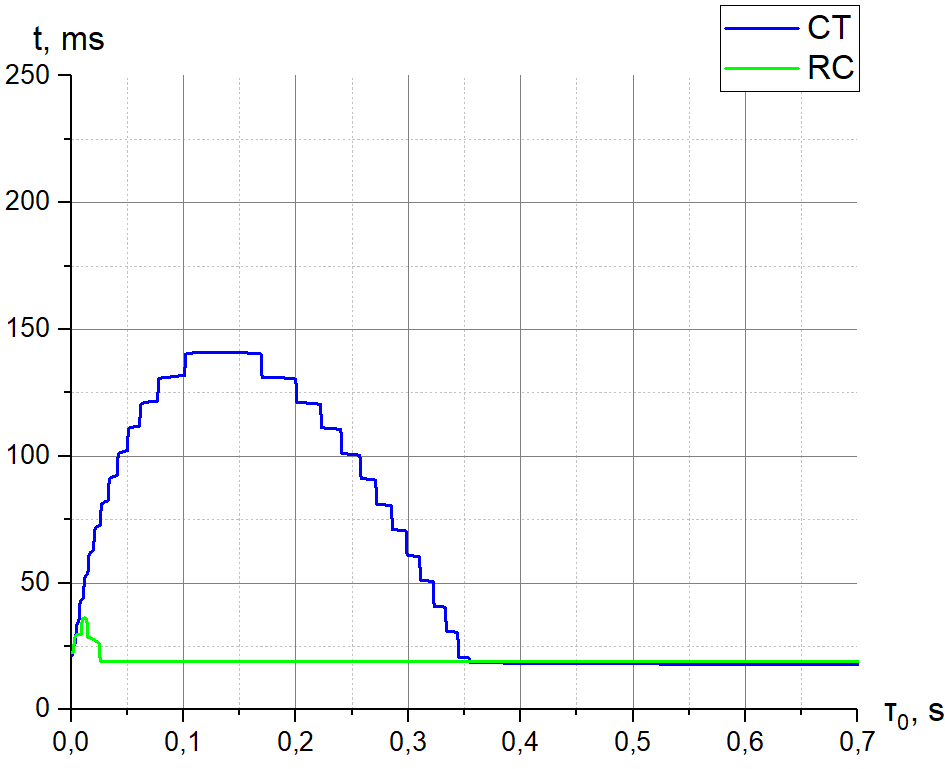
\includegraphics[width=0.46\textwidth]{image62.png} \\
    а) & б) \\
    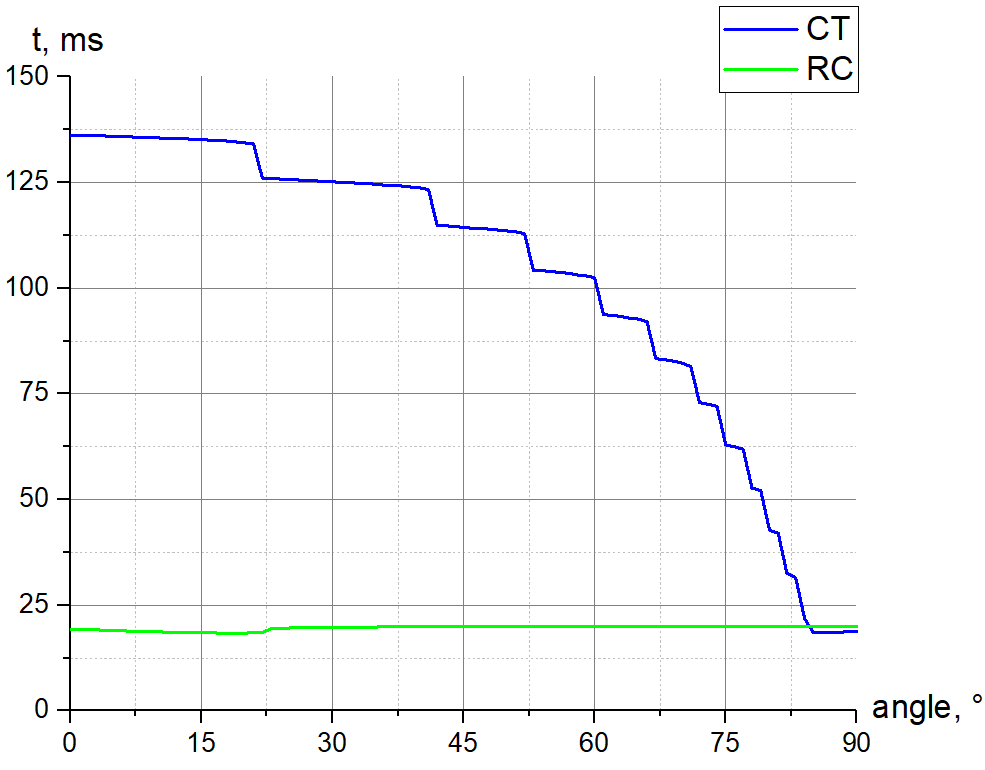
\includegraphics[width=0.46\textwidth]{image63.png} & 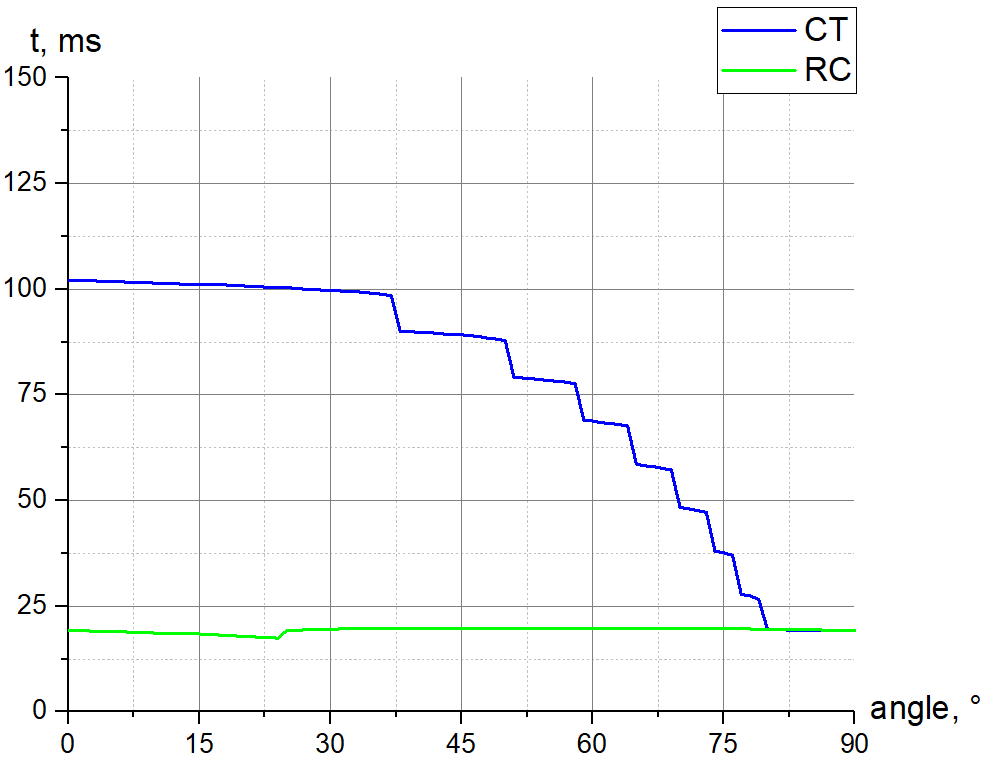
\includegraphics[width=0.46\textwidth]{image64.png} \\
    в) & г)
  \end{tabular}
  \caption{Время переходного процесса:\\
  -- при различном времени затухания апериодической составляющей: а) определяемое по модулю, б) определяемое по углу;\\
  -- при различном начальном угле КЗ: в) определяемое по модулю, г) определяемое по углу}
  \label{fig:ch02_transient_time_factors}
\end{figure}

% DISS-005-B0837
\subsection{Влияние высших гармоник}
\label{sec:ch02_higher_harmonics}

% DISS-005-B0838
Напряжение на выходе КР пропорционально производной тока. При одинаковой амплитуде тока вклад гармоники в выходное напряжение возрастает с её частотой. Поэтому оценено влияние высших гармоник на амплитуду и угол первой гармоники, рассчитываемые по сигналу КР.

% DISS-005-B0839
Исследуемый ток содержал вторую, третью и десятую гармоники с относительными амплитудами $h_2=0{,}3$, $h_3=0{,}2$ и $h_{10}=0{,}1$ соответственно. Вторая и третья гармоники моделировали искажения при насыщении магнитопроводов силового оборудования, десятая представляла высокочастотную составляющую испытательного сигнала. Начальный угол КЗ всех гармоник принят равным нулю, что соответствует наибольшему модулю апериодической составляющей\commentnote{DISS-005-C0083}{Valery Valery}{Это слово хорошо переведется на английский, но оно просто ужасно))}. Формулы используемых сигналов приведены ниже~\eqref{eq:ch02_harmonics_signals}.

(Примечание автора: Закрываем примечание 10 и не надо ответа на это сообщение)

% DISS-005-B0840
% DISS-005-B0841
% DISS-005-B0842
\begin{equation}
\label{eq:ch02_harmonics_signals}
\begin{aligned}
i(t) &= \sqrt{2}I_{\text{кз}}\left(A_0 e^{-t/\tau_0}-f(t)\right),\\
f(t) &= \cos(\omega t+\varphi_{\text{КЗ}})
     - \sum_{n\in\{2,3,10\}} h_n \cos(n\omega t+\varphi_{\text{КЗ}}),\\
i'(t) &= \sqrt{2}I_{\text{кз}}
         \left(-\frac{A_0}{\tau_0} e^{-t/\tau_0}-f'(t)\right),\\
f'(t) &= -\omega\sin(\omega t+\varphi_{\text{КЗ}})
       + \sum_{n\in\{2,3,10\}} n\omega h_n \sin(n\omega t+\varphi_{\text{КЗ}}).
\end{aligned}
\end{equation}

% DISS-005-B0843
Коэффициент $A_0=(1+h_2+h_3+h_{10})\cos\varphi_{\text{КЗ}}$ задаёт апериодическую составляющую исходного сигнала. Множитель $\sqrt{2}I_{\text{кз}}$ равен амплитуде первой гармоники тока, $\tau_0$ обозначает постоянную времени затухания, $\omega$ обозначает угловую частоту первой гармоники, $t$ обозначает время от начала переходного процесса. Безразмерная функция $f(t)$ описывает периодическую часть с учётом знака перед ней в выражении тока. Множители $n\omega$ возникают при дифференцировании гармоник. Величины $i(t)$ и $i'(t)$ измеряются соответственно в амперах и амперах в секунду.
\figurereview{Сверить начальное условие со схемой генерации сигналов. При записанных знаках $i(0)=2\sqrt{2}I_{\text{кз}}(h_2+h_3+h_{10})\cos\varphi_{\text{КЗ}}$. Что задано в модели: ненулевой ток до КЗ, иной знак высших гармоник или иной коэффициент экспоненты?}

(Примечание автора: Есть такое чувство, что специально были заданы высшие гармоники с "минусом", надо бы прост проверить график, который получается, он наверное не тут, а в матлабе строился. Но здесь можно будет быстренько его прогнать, построить и глянуть картинку, чтобы совпадала. А по тексту – тогда надо будет поправить описание… Хотя может и не надо править описание, угол же и правда везде 0-ой. В общем, противоречия тут надо проверить построив график и посмотрев, какой будет больше подходить под реальность, может и правда прост опечатка в записи и первичный косинус тоже должен был быть с минусом. Изучи этот момент и сделай правильно под график.)

% DISS-005-B0844

% DISS-005-B0845
% DISS-005-B0846
\begin{figure}[htbp]
  \centering
  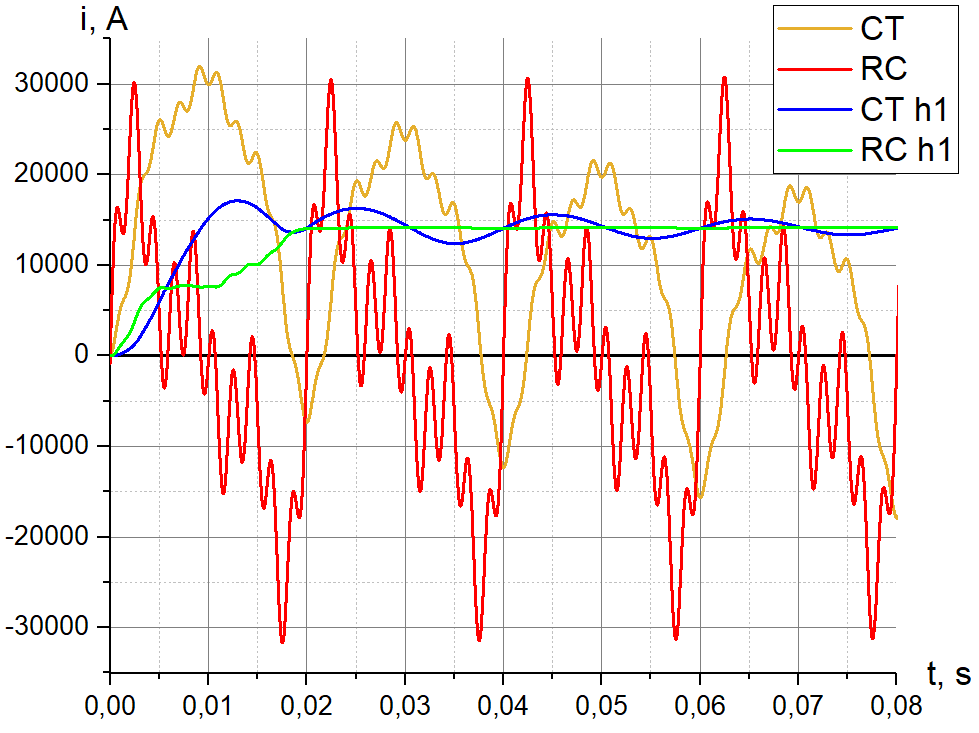
\includegraphics[width=0.88\textwidth]{image65.png}
  \caption{Исследуемые сигналы с ТТ без учёта насыщения и КР с наличием 2, 3, и 10 гармоник в сигнале; и рассчитанные амплитуды первой гармоники.}
  \label{fig:ch02_harmonics_currents}
\end{figure}

% DISS-005-B0847
Рисунок~\ref{fig:ch02_harmonics_currents} показывает исходные сигналы и рассчитанные по ним амплитуды первой гармоники. Как можем видеть, наличие высших гармонических составляющих для КР вносит дополнительное искажение только на первом периоде расчёта, далее амплитуда остаётся стабильной. Данное поведение и ожидалось, так как описанные неточности измерения обусловлены апериодической составляющей, которая лишь немного изменилась по амплитуде.

% DISS-005-B0848
\subsection{Ускорение работы алгоритмов на начальном участке и применение КР для алгоритмов на мгновенных значениях}
\label{sec:ch02_instantaneous_values}

% DISS-005-B0849
Как можно было заметить ранее, на начальном участке значение амплитуды первой гармоники, рассчитанное на основе сигнала с катушки Роговского, опережает аналогичное значение с идеальных классических ТТ (Рисунок 2.9). Данный фактор может быть полезен при функционировании быстродействующих устройств РЗА и БАВР в первые моменты развития аварии.

% DISS-005-B0850
% DISS-005-B0851
% DISS-005-B0852
% DISS-005-B0853
% DISS-005-B0854
\begin{figure}[htbp]
  \centering
  \begin{tabular}{cc}
    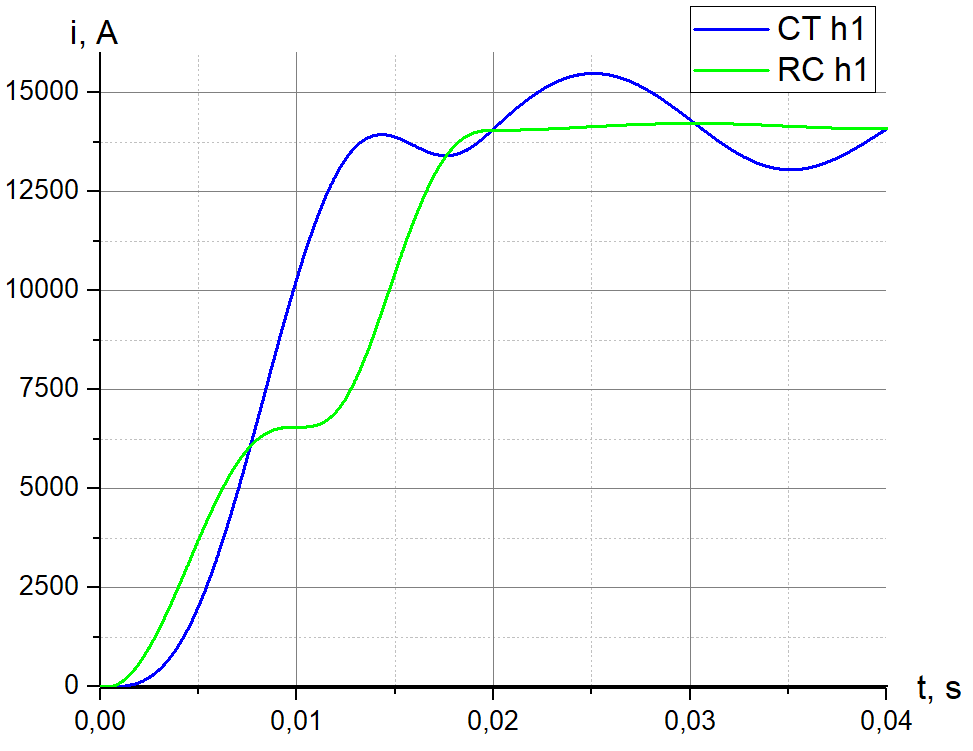
\includegraphics[width=0.48\textwidth]{image66.png} & 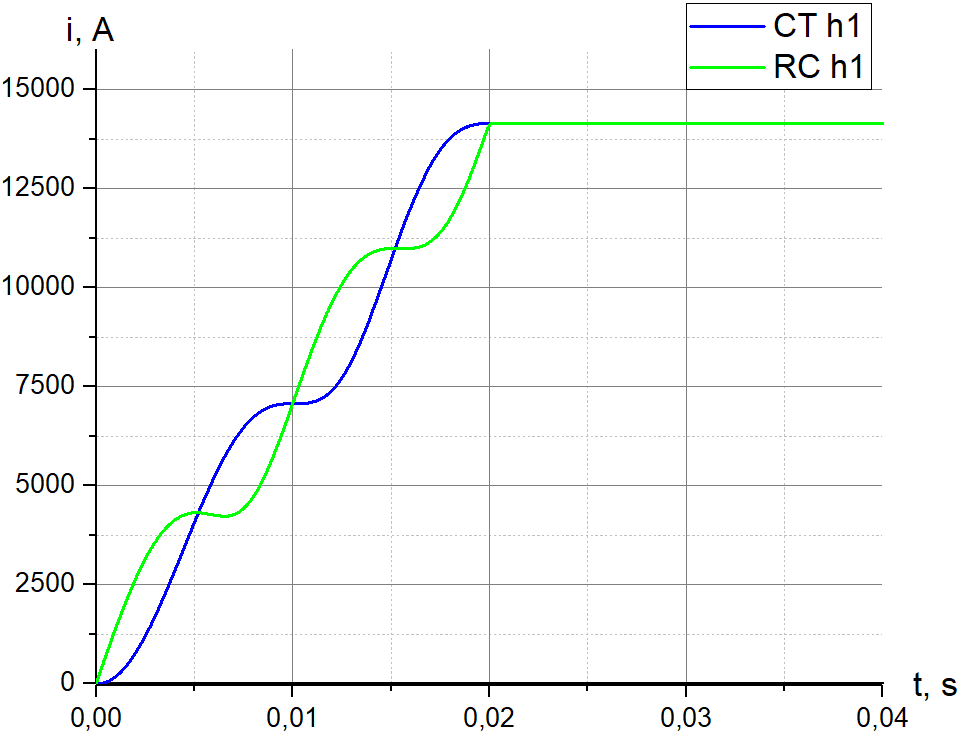
\includegraphics[width=0.48\textwidth]{image67.png} \\
    а) & б)
  \end{tabular}
  \caption{Переходный процесс, амплитуды первой гармоники: а) при максимальной доле апериодической составляющей и постоянной времени 50~мс, б) при отсутствии апериодической составляющей}
  \label{fig:ch02_initial_transient}
\end{figure}

% DISS-005-B0855
Алгоритмы получения амплитуды сигнала, основанные на мгновенных значениях [22]\commentnote{DISS-005-C0084}{Алексей Евдаков}{Добавил одну работу, по-хорошему бы ещё добавить методичку, по которой делается лабораторная, о которой говорил Андрей.}\commentnote{DISS-005-C0085}{Евдаков Алексей}{Эту статью надо обновить / вставить.}, могут быть использованы для ускорения функционирования устройств. \commentnote{DISS-005-C0086}{Андрей Яблоков}{Не надо начинать предложения с также}Если для классических ТТ у данных подходов возникают существенные погрешности при апериодической составляющей, то для катушек Роговского данный эффект практически отсутствует ввиду её подавления физической природой датчика.

(Примечание автора: Закрываем примечание DISS-005-C0084, DISS-005-C0085, DISS-005-C0086 и не надо ответа на это сообщение)
(Примечание автора: Раньше я писал не такими кодами, извини, надеюсь разберёшься, что имел ввиду раньше, все предыдущие как раз шли рядом с подобными замечаниями. Ответа на сообщение не нужно, прост закрой его.)

% DISS-005-B0856
Таким образом, применение катушек Роговского в устройствах релейной защиты и автоматики обеспечивает:
\begin{itemize}[noitemsep,topsep=2pt]
% DISS-005-B0857
\item Устойчивость работы защит за счет исключения насыщения, характерного для ТТ.
% DISS-005-B0858
\item Снижение влияния апериодической составляющей на расчет первой гармоники.
% DISS-005-B0859
\item Сокращение времени расчётного переходного процесса, что критично для быстродействующих защитных устройств.
% DISS-005-B0860
\item Экономическую эффективность и простоту монтажа, особенно при модернизации существующих подстанций.
\end{itemize}

% DISS-005-B0861
При этом совместное использование сигналов с классических ТТ и КР является интересной идей для поиска баланса между данными типами датчиков. В дальнейшем предлагается использовать нелинейную зависимость, при которой на малых токах приоритет отдается сигналу с ТТ для повышения точности за счет исключения шумов, а при больших - сигналу с КР для компенсации насыщения сердечника ТТ. Такая концепция может быть применима, например, на цифровых, так как приём сигнала по SV потоку не требует прокладки дополнительных кабелей. Разные типы датчиков могут присутствовать в комбинированных измерительных приборах, например: ТТ используется для измерений, а КР~-- для целей РЗА.
